\documentclass{frontiersSCNS}

%%%%% Some customizations

\usepackage{listings}
\usepackage{inconsolata}

\definecolor{dkgreen}{rgb}{0,0.6,0}
\definecolor{gray}{rgb}{0.5,0.5,0.5}
\definecolor{mauve}{rgb}{0.58,0,0.82}

\lstset{
  language=Python,
  aboveskip=3mm,
  belowskip=3mm,
  showstringspaces=false,
  columns=flexible,
  basicstyle={\small\ttfamily},
  numbers=none,
  numberstyle=\tiny\color{gray},
  keywordstyle=\color{blue},
  commentstyle=\color{dkgreen},
  stringstyle=\color{mauve},
  breaklines=true,
  breakatwhitespace=true,
  deletendkeywords={filter},
}

\graphicspath{{figures/}}

%%%%% Frontiers boilerplate

\usepackage{url,lineno}
% \linenumbers  % TODO uncomment!

\copyrightyear{2013}
\pubyear{2013}

\def\journal{Neuroinformatics}
\def\DOI{}
\def\articleType{Methods Article}
\def\keyFont{\fontsize{8}{11}\helveticabold }
\def\firstAuthorLast{Bekolay {et~al.}}
\def\Authors{Trevor Bekolay\,$^{1,*}$, James Bergstra\,$^{1}$,
  Xuan Choo\,$^{1}$, Travis DeWolf\,$^{1}$, Eric Hunsberger\,$^{1}$,
  Daniel Rasmussen\,$^{1}$, Terrence C. Stewart\,$^{1}$
  and Chris Eliasmith\,$^{1}$}
\def\Address{$^{1}$Computational Neuroscience Research Group,
  Center for Theoretical Neuroscience,
  University of Waterloo, Waterloo, ON, Canada}
\def\corrAuthor{Trevor Bekolay}
\def\corrAddress{David R. Cheriton School of Computer Science,
  University of Waterloo, 200 University Avenue West,
  Waterloo, ON, N2L 3G1, Canada}
\def\corrEmail{tbekolay@uwaterloo.ca}

%%%%% Document begins

\begin{document}
\onecolumn
\firstpage{1}

\title[Nengo in Python]{Nengo: A Python tool for
  building large-scale functional brain models}
\author[\firstAuthorLast ]{\Authors}
\address{}
\correspondance{}
\extraAuth{}
%\extraAuth{corresponding Author2 \\ Laboratory X2, Institute X2, Department X2,
%  Organization X2, Street X2, City X2 , State XX2
%  (only USA, Canada and Australia), Zip Code2, X2 Country X2, email2@uni2.edu}
\topic{Python in Neuroscience II}

\maketitle

\begin{abstract}
%Maximum: 2000 characters

  \tiny \keyFont{\section{Keywords:} 1 2 3 4 5 (6 7 8)}
\end{abstract}

%max figures+tables: 15
%max legnth: 12000 words
%max pdf length: 12 pages

\section{Introduction}

It is often said that neuroscience
is data-rich but theory-poor.
Although computational neuroscience
has grown significantly,
this phrase continues to be repeated
due to a lack of satisfying
theories of the brain.
Much work has been put into neural simulators
that attempt to recreate neuroscientific
data in precise detail,
but behavior has not emerged
from data-driven large scale models.
Similarly, theoretical frameworks
consisting of a generic algorithm
replicated many times
(e.g., the memory-prediction framework \cite{TODO}
and the pattern recognition theory of mind \cite{TODO})
have not been shown to solve problems
that the generic algorithm alone cannot solve.

Nengo is a neural simulator
based on a theoretical framework proposed
by Eliasmith \& Anderson \citeyearpar{TODO}
called the Neural Engineering Framework
(NEF).
Nengo was recently used to implement Spaun,
currently the world's largest functional brain model
\cite{TODO}.
Spaun is a network of 2.5 million spiking neurons
that can perform eight high-level cognitive tasks
including list memory and inductive reasoning.
It can perform any of these eight tasks
at any time by being presented
the appropriate series of images
representing the task to be performed
and the details of that task;
for example, sequentially presenting images
containing the characters $A3[1234]$ instructs Spaun
to remember the list $1234$.
It then provides its answer by
sending motor commands to a simulated arm model,
tracing out digits.
If asked to recall the remember list,
it would trace out the digits $1234$.

While the tasks Spaun performs are diverse,
all tasks use a common set of
functional modules that we map
onto the brain areas hypothesized
to perform those functions.
Like data-driven large scale models,
Spaun is able to match experimental data
across the neuroscientific spectrum,
from the single cell to the behavioral level.
However, instead of constructing the model
based on data and hoping behavior emerges,
we construct the model
based on behavior
and see that the data emerges.
This is made possible by a theoretical framework
like the memory-prediction framework \cite{TODO},
but unlike it and other frameworks,
the NEF enables Spaun to employ
many different algorithms
based on the behavior being performed,
rather than defining a single algorithm
and hypothesizing that replicating it
many times will enable these behaviors.

In implementing Spaun,
we provided strong support
that the NEF is beginning to fill the theory void in neuroscience.
However, in doing so, we pushed Nengo
to the limits of its ability to construct and simulate
large-scale neural models.
In order to continue to evaluate the NEF
as a theory of the brain
by building larger and more complicated models,
we have begun the next generation
of Nengo with a focus on speed,
extensibility, and simplicity.

\subsection{JavaNengo limitations}

\begin{table}[!t]
\processtable{Nengo tools\label{tab:nengo-vers}}
{\begin{tabular}{p{2.6cm} p{2.7cm} l p{7cm}} \toprule
\textbf{Name} & \textbf{Implementation language}
  & \textbf{Code repository} & \textbf{Purpose} \\\midrule
JavaNengo simulator & Java & \texttt{nengo\_java}
  & Simulates many types of spiking neuron models.
  Includes methods to construct and simulate models using the NEF. \\
JavaNengo GUI & Java & \texttt{nengo\_java\_gui}
  & Graphical interface to JavaNengo simulator.
  Allows modellers to drag-and-drop components built with the NEF. \\
JavaNengo scripting interface & Jython & \texttt{nengo\_jython}
  & Scripting interface to JavaNengo simulator.
  Provides shortcuts to classes and functions in the simulator.
  Also accessible through and interacts with the JavaNengo GUI. \\
PyNengo & Python & \texttt{nengo}
  & Constructs and simulates models using the NEF. \\
PyNengo OpenCL simulator & Python+PyOpenCL
  & \texttt{nengo\_ocl}
  & Simulates models constructed with PyNengo. \\\botrule
\end{tabular}}{Code repositories avilable at \url{http://github.com/ctn-waterloo/}}
\end{table}

JavaNengo is a suite of tools providing
a neural simulator and graphical user interface (GUI)
implemented in Java,
and a scripting interface implemented in Jython
(see Table~\ref{tab:nengo-vers} for more detail).
JavaNengo's simulator was created
with the intention of being a general
neural simulator that included
the methods of the NEF
as one of several
methods for creating neural models.
As a result, its implementation
of important NEF components
are nested in deep class hierarchies,
adding unnecessary layers of complexity
for developers wishing
to extend those NEF components.
As a representative example,
the most often used class for making
NEF models, \texttt{NEFEnsemble},
extends from five ancestor classes
and implements seven interfaces.
Adding support for synaptic plasticity
in \texttt{NEFEnsemble}
involved adding or significantly modifying
25 Java classes \cite{TODO}.

The JavaNengo GUI provided
a drag-and-drop interface in which to create NEF models.
However, as it was developed
before the scripting interface,
the GUI manipulates simulator objects directly.
Typically, modellers start by following
tutorials that use the GUI interface,
and transition to the scripting interface
in order to implement more complicated models.
Since the GUI modifies simulator objects directly,
modelling concepts learned in the GUI
have to be relearned in the scripting interface.

The JavaNengo scripting interface,
described in \cite{TODO},
provided a simpler interface
to the NEF-specific portions of the simulator.
This greatly enhanced productivity,
and made it possible
to create many models with very little code.
Modellers quickly started using
the scripting interface
as their primary tool,
but still needed to access the GUI
for interactive model inspection,
and still needed to modify the simulator
to add new functionality
(e.g., to add new neuron models).
This is because Jython makes it easy
to inspect and create Java objects,
but does not make it easy to
write Java code to
inspect and create Jython objects.
Modellers, therefore, had to be
proficient in Java whether
they used the scripting interface or not.
As there are few neural modellers
that are proficient with both Java and Python syntax,
the scripting interface still lacks
convenient ways to record the results of simulations,
and to define complex experimental setups.

Finally, perhaps the most significant limitation
of the JavaNengo tools is their performance.
While Java has good support for threads,
it does not have well-supported libraries
for doing mathematical operations on large matrices quickly.
Additionally, it is difficult to interface with
platform-specific tools such as
graphical processing units (GPUs),
which can perform the types of computations
that neural models require quickly and in parallel.

Addressing all of these issues
in the Java codebase would involve
significant enough changes
that we started from scratch instead.
Since the scripting interface
already used Python syntax,
and since Python is widely used
for neuroscientific data analysis,
we targeted the CPython interpreter
as the platform for the next generation of Nengo.

\subsection{PyNengo}

PyNengo,
the subject of the remainder of this paper,
is a Python package for
defining and simulating
neural models using the NEF.
It targets the CPython interpreter,
meaning that it integrates seamlessly
with other scientific Python tools.
Arbitrary CPython programs
can use Nengo models,
opening up possibilities
for using neurally implemented algorithms
in applications and games.

PyNengo's object model is simple and minimal,
making it easy to
document, test, and modify.
It also includes a scripting interface to those objects
based on JavaNengo's scripting interface \cite{TODO},
but with several modifications
to allow for easier incorporation
of user-defined networks,
new neuron models, and learning rules.
Additionally, PyNengo's scripting interface
contains methods to record simulated data
and access that data after simulation.

Model creation and simulation are decoupled,
allowing for models to be exported
to other simulators,
such as those accessible with PyNN.
Simulators can also be written
to leverage specific platforms.
Currently, we have implemented
a platform-independent simulator
that uses NumPy for vectorized computations,
and a PyOpenCL-based
simulator that takes full advantage of GPUs
and multicore CPUs.

PyNengo does not currently
replace all of JavaNengo's functionality.
While it can simulate the vast majority
of models that JavaNengo can simulate,
some functionality is still in development.
Most notably, there is no graphical interface
to PyNengo, and therefore simulations
cannot be visualized while they are running.
However, we are confident that these tools
can be created, and will be much easier
to implement compared to JavaNengo's GUI.

PyNengo overcomes all of JavaNengo's limitations.
It can simulate most models
currently simulated by JavaNengo
using 11\% as many lines code,
and depending on
only three external libraries instead of ten.
The OpenCL simulator can simulate
a large model TODO times
faster than JavaNengo's simulator.
This, along with a codebase
that is well tested and
easy to understand and extend,
provides a platform
that can simulate larger and more complex
models than Spaun,
and can therefore further
test the NEF as a theory of the brain.

\section{Neural Engineering Framework (NEF)}

The Neural Engineering Framework (NEF; \cite{TODO})
proposes three principles
that enable the construction
of large-scale neural models.

\begin{enumerate}
  \item \textbf{Representation:} A population of neurons
    collectively represents information in the form of
    time-varying vectors of real numbers.
  \item \textbf{Transformation:} Functions on those vectors
    are computed by the connections between populations.
  \item \textbf{Dynamics:} The vectors represented
    by neural populations can be considered state variables
    in a dynamical system, and can be analyzed using control theory.
\end{enumerate}

\begin{figure}
\begin{center}
  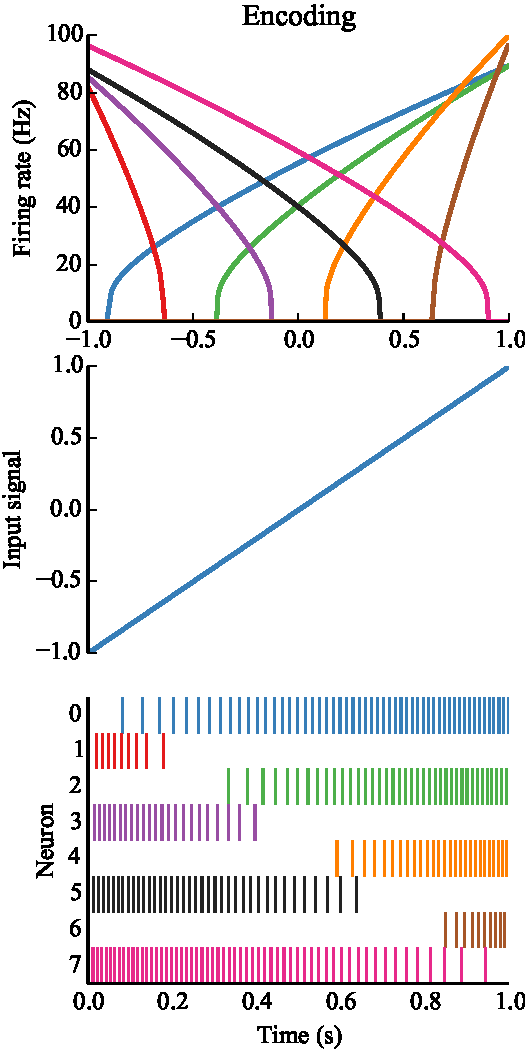
\includegraphics[width=0.19\textwidth]{nef_summary_enc}
  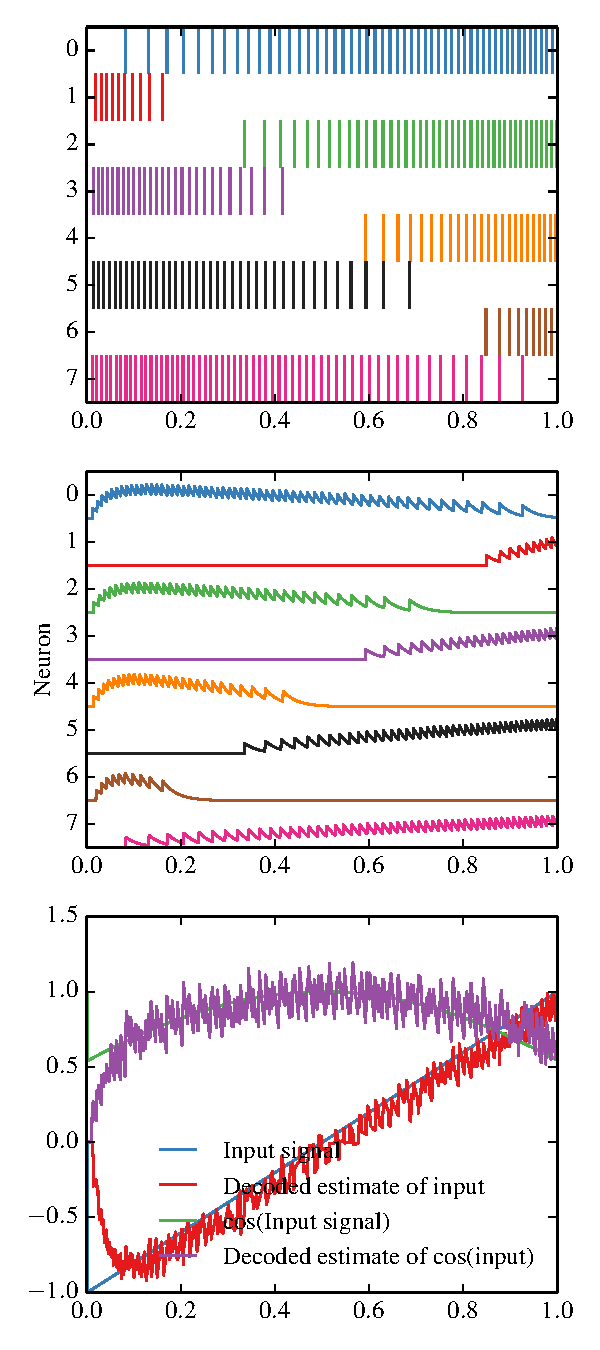
\includegraphics[width=0.19\textwidth]{nef_summary_dec}
  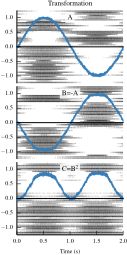
\includegraphics[width=0.399\textwidth]{nef_summary_trans}
  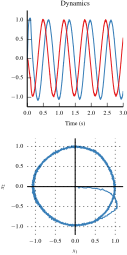
\includegraphics[width=0.199\textwidth]{nef_summary_dyn}
\end{center}
 \textbf{\refstepcounter{figure}\label{fig:nef} Figure \arabic{figure}.}{
   Summary of the Neural Engineering Framework.}
\end{figure}

\paragraph{Representation}
Information is encoded by populations of neurons.
We consider that information
to be time-varying vectors of real numbers,
in order to reason with that information
using conventional mathematics.
By doing this, we can \textit{encode}
those vectors by injecting
specific amounts of current into
single neuron models based on
the vector being encoded.
This drives the neuron,
causing it to spike.
We can then estimate
the originally encoded vector
through a \textit{decoding} process.
This idea is similar to population coding
\cite{TODO}, but generalized
to vectors of arbitrary length.

Figure~\ref{fig:nef} depicts
the encoding (A) and decoding (B) process.
In the encoding process, the input signal drives
each neuron based on its \textit{tuning curve},
which describes how much
that neuron fires for a given input signal.
The tuning curve summarizes the gain
of a neuron (how quickly the activity rises),
the bias (the activity of a neuron given no signal),
and the encoding weight
(the part of the vector space
that causes the neuron to fire most strongly).
This results in a predictable pattern of firing
given the input signal.

In the decoding process,
the spike trains are first filtered
with an exponentially decaying filter.
Those filtered spike trains are summed together
with weights that are determined
by solving a least-squares minimization problem.
In the bottom panel of Figure~\ref{fig:nef}B,
the red line is the filtered spiking activity
weighted by decoding weights
that minimize the difference between
the actual encoded vector
and the decoded estimate.
The purple line is the filtered spiking activity
weighted by decoding weights
that minimize the different between
the cosine of the actual encoded vector
and the decoded estimate.
Note that these decoding weights are not determined
based on the input signal;
instead, the minimization occurs
on points that are randomly sampled
in the vector space
that the population represents.

\paragraph{Transformation}
Neurons communicate through
unidirectional connections called synapses.
When a neuron spikes,
it releases neurotransmitter across the synapse,
which causes some amount of current
to be imparted in the downstream neuron.
Many factors affect the
amplitude of the current imparted;
we summarize those factors
in a scalar connection weight
representing the strength
of the connection between two neurons.
In order to compute any function,
we can set the connection weights between
two populations to be the product of
the decoding weights for that function
for neurons in the first population
and the encoding weights
for the downstream neuron.

In Figure~\ref{fig:nef}C,
a sine wave is transformed twice.
Between populations A and B,
the signal is negated.
Between populations B and C,
the signal is squared.

Note that, in practice, we rarely use
the full connection weight matrix,
and instead store
the encoding and decoding weights
(i.e., the factors of the connection weight matrix).
This provides significant
space and time savings.

\paragraph{Dynamics}
While doing feedforward transformations
on vectors is sufficient to model
many neural systems,
many systems, notably memory systems,
require persistent activity through recurrent connections.
When recurrent connection are introduced,
the vectors that populations represent
can be thought of as state variables
in a dynamical system.
Neural systems can therefore
be built and analyzed using
the methods of control theory.

In Figure~\ref{fig:nef}D,
a population represents a two-dimensional vector,
and is recurrently connected
with negative feedback between dimensions,
resulting in a harmonic oscillator.

\paragraph{Nengo}
Large models can be built
by thinking of the principles of the NEF
as building blocks that can be put together
to describe neural systems.
The goal of Nengo is to allow
modellers to describe neural systems
in terms of what information is being represented,
how that information is transformed,
and what dynamics are required
to perform cognitively relevant
functions with biologically constrained
neural components.
Those descriptions are then
translated to a network
of interconnected neurons.
This situates Nengo
as a ``neural compiler''
that translates
a high-level functional model
to a low-level neural model
that implements the high-level function.

\section{PyNengo object model}

\subsection{Model}

A Nengo model is a collection
of Nengo objects that represent information
and connections that transform information.
Objects and connections can be probed
in order to collect data during simulation.

The \texttt{Model} object is primarily a container
for Nengo objects,
but also doubles as
a scripting interface
that simplifies creating, connecting,
and probing objects.
Basic models
can be created solely through interacting
with the \texttt{Model} object
(see sections \ref{sec:comm-channel}--\ref{sec:lorenz}
for examples).
In advanced models,
objects are instantiated
and then added to the model
(see section \ref{sec:cconv} for an example).

\subsection{Ensemble}

An \texttt{Ensemble} is
a population of neurons
that represents information
in the form of a real-valued vector.
An ensemble must be given as arguments
its dimensionality
(i.e., the length of the vector it represents),
and an object that describes
the population of neurons.
For example, \texttt{nengo.LIF(50, tau\_ref=0.002)}
describes a population
of 50 leaky integrate-and-fire neurons
with a refractory time of 0.002 seconds.
Neurons are defined symbolically
so that each simulator can compute
this population's nonlinear function
however it sees fit.
The neuron model used by the population
is easily changed, as long as the simulat

Other attributes of the \texttt{Ensemble},
such as its encoding weights, $\mathbf{e_i}$,
the maximum firing rate of the neurons,
and so on, can also be specified.
This is usually done according
to what is known about
the neurobiology of the area being modelled;
some areas of the brain regularly spike
at rates above 200Hz,
while others rarely spike above 10Hz.
If these attributes are not set,
then they will be randomly selected
from distributions that describe
what is known about pyramidal cells in neocortex.

\subsection{Node}
A \texttt{Node} tracks any information
that is not represented by an ensemble.
In the most common case,
nodes provide input signals
that drive ensembles of sensory neurons.
In a more general sense,
nodes represent the experimental environment
in which a neural model exists.
More practically,
nodes can be used to directly compute
parts of a neural model
for debugging purposes.

A node computes an arbitrary function
of its inputs directly.
Possible input signals include
the simulator timestep,
the decoded output of an ensemble,
or the output of another node.
However, unlike ensembles,
there are no constraints on the type
of function that the node computes.
A node can track any number of variables internally,
and use the state of those variables
when computing its function.
It can interact directly with hardware,
interface with other programs
using shared memory or sockets,
and so on.

Nodes allows many of the special-purpose
routines that are necessary in many real-world
models to be integrated
as core components of a Nengo model.

\subsection{Connections}

Ensembles and nodes can be connected together
in several ways.
Like other high-level objects,
a connection contains symbolic information
about how two objects are to be connected
together.

The most important type of connection
in Nengo is the \texttt{DecodedConnection}.
This connection implements
the transformation principle equations,
\eqref{TODO}.
In other words, the \texttt{DecodedConnection}
allows ensembles to project
the information they're representing---or
a transformation of that information---to
another ensemble or node.
This functionality is what enables Nengo models
to appear conceptual,
even though the underlying implementation
still connects populations of neurons
together with connection weights.

\subsection{Probes}

Ideally, the entire state of a simulation
would be recorded on each timestep,
and stored with no overhead to the simulator.
In practice, recording data
is a costly part of most simulations,
and often what is simulated must also change
if the signals being probed must be filtered.
For this reason, probes are also
a core component of a Nengo model.

In general, Nengo objects and connections
each have several signals that can be probed.
For example, an ensemble's decoded value,
or the underlying neurons' membrane voltages
can be probed, among other signals.
The underlying logic for the probe
leverages connection logic,
making it easy to probe any part of an object.

Since probes are also described
at a symbolic level,
the underlying implementation
can output probed data in many different formats.
Currently, simulators store probed data
directly in memory,
but adding the ability to store data
in files or to stream probed data
directly to sockets will be added.

\subsection{Networks}
A network is a collection of ensembles and nodes
connected together in a particular way.
It is primarily a way of grouping together
a common set of objects connected in a particular way,
and provides some implicit expressiveness
in the name of the network.

Networks can vary dramatically in size,
and can be composed of other networks.
The \texttt{Integrator} network, for example,
is composed of only one recurrently connected ensemble.
By encapsulating that logic in a network,
the purpose of that ensemble is made explicit.
On the other end of the size spectrum,
the \texttt{BasalGanglia} network,
is composed of five groups of ensembles
connected with several specific functions
that together implement a ``winner take all'' circuit.
Encapsulating that logic
makes this complicated section of code
easy to include in many different models
(see Figure~\ref{TODO}).

\section{PyNengo simulators} \label{sec:simulators}

Once a model has been fully defined,
a simulator can be created to
run that model.
Simulators can be created
that work directly with the
objects described in section \ref{sec:objects}.
However, in the simulators that we have implemented
as reference, the model goes through a
two-stage build process in order to
simulate models as fast as possible.
In the first stage,
the model is ``built;''
i.e., the objects in the model are mapped to a simpler
set of objects that represent the computations
that the simulator must perform.
Those computations are analyzed in order to
schedule them efficiently.
In the second stage,
the simulator performs the computations
that have been scheduled on each timestep.

This two-stage process has enabled us
to implement a more efficient simulator
that is only aware of
the objects that are created
during the build process.
In the future,
new simulators can target either
the high level Nengo objects,
or the low level simulator objects
depending on the constraints of the platform.

\subsection{Reference build process}

\begin{figure}
\begin{center}
  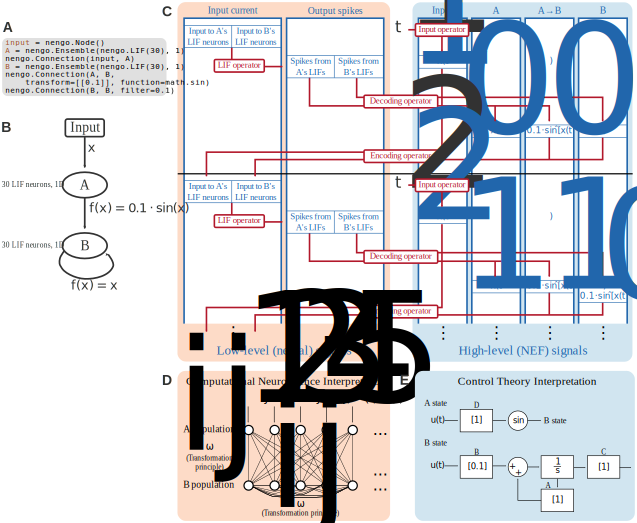
\includegraphics[width=0.6\textwidth]{sim}
\end{center}
 \textbf{\refstepcounter{figure}\label{fig:sim} Figure \arabic{figure}.}{
   Sim}
\end{figure}

The first stage of the reference implementation
maps all of the Nengo objects
down to a set of signals and operators.

\paragraph{Signals}
A \texttt{Signal} represents any number that
will be used by the simulator.
Each high level Nengo object contains
several signals;
for example, an ensemble contains signals
that represent the high-level input
signal that will be encoded
to input currents (see equation \eqref{TODO}),
and the encoding weights
($\mathbf{e_i}$; see equation \eqref{TODO}).
It also contains a neural population,
which contains signals that represent
input currents
($J(t)$; see equation \eqref{TODO}),
bias currents ($J^{bias}$; \eqref{TODO}),
membrane voltages ($V$; \eqref{TODO}),
and refractory times for each cell.
These signal are symbolic,
and contain only information
about the size of the signal that will be represented,
and optionally an initial value.
Simulators may therefore represent
these signals however they want internally.

In some cases, determining
the initial values of some signals
may involve some computation.
In particular, solving for decoding weights
(equation \eqref{TODO}) requires
solving a least-squares minimization problem.
This computation is done in this stage
of the build process,
as it is computationally intensive,
and may be implemented
differently by some simulators.

An important feature of signals
is that parts of a signal
can be accessed with Python slice syntax,
which results in a view of the original signal.
For example, when connecting to
a subset of a population of neurons,
current would be injected
in a view of the overall input current signal
for that population,
rather than creating a new signal,
or partitioning the population's signal
into smaller chunks.
Grouping related signals together
and exposing them through views
also provides hints to the simulator
that can be used to organize signals
efficiently in memory.

\paragraph{Operators}
Operators represent computations
to be performed on signals on each timestep.
Once the model has been built,
only a small set of mathematical
operations are necessary for simulation.
\begin{enumerate}
  \item \textbf{Reset} assigns a constant value to a signal.
    This is typically used to set a signal to 0
    at the start of a timestep.
  \item \textbf{Copy} assigns the value
    of one signal to another signal.
    This is typically used instead of \textbf{Reset}
    in situations where the signal's value
    at the start of a timestep should
    be the value of another signal.
  \item \textbf{DotInc} increments a signal by
    the dot product of two signals;
    i.e., $Y \leftarrow Y + AB$.
    This is a common operation
    done in many situations,
    such as decoding a signal (see equation \eqref{TODO}).
  \item \textbf{ProdUpdate} scales a signal
    and adds the dot product of two signals to it;
    i.e., $Y \leftarrow BY + AX$.
    This is done when temporally filtering a signal.
  \item \textbf{Nonlinearities} include any
    user-defined function computed by a node,
    and the update equation for each neuron model.
\end{enumerate}

It is important to note that all operators
excepts for the nonlinearities are linear,
and therefore can share an implementation
in an underlying simulator,
allowing those operations to happen in parallel.

Operators are created
by Nengo objects during the build process.
For example, an ensemble creates
a \textbf{Reset} operator to reset
its input signal to 0,
and a \textbf{DotInc} operator
to encode that input signal into
input currents injected into
the underlying population of neurons;
i.e., the \textbf{DotInc} computes
$J = \alpha_i \mathbf{e_i} X$ from equation \eqref{TODO}.

\subsection{Reference simulator}

The reference simulator starts by
building NumPy arrays
for every signal created during the build process
described above.
It then builds a graph of the
operators created during the build process,
ordering them such that they can be
executed one after another to get the correct answer.

The ordering is determined
by which signals an operator
sets, increments, reads, and updates.
A signal can only be set or updated once,
but can be read or incremented any number of times.
An update represents the operator that sets
the signal's value at time $t+dt$,
and therefore must be the last operator
that acts on a given signal.
This means that an operator
that updates a signal depends on
all operators that set, increment,
or read that signal.
Reads represent reading the value
of a signal at time $t$,
which is determined by the sets
and increments, and so
an operator that reads a given signal
depends on all operators that
set and increment that signal.
Increments must happen
after a given signal is set,
so an operator that increments a given
signal depends on the operator
that sets that signal, if it exists.

The reference simulator represents
these dependencies by a directed graph,
with edges going from
dependent operators to
the operators on which they depend.
The dependency graph is then topologically sorted,
and that ordering is stored.

The simulator can then be run
for an arbitrary amount of time.
On each timestep,
the simulator goes through each of the
operators in order,
and then makes a copy of any signals
that were probed on this timestep.

\subsection{OpenCL simulator}

OpenCL is a framework for writing
efficient parallel code that runs
on many different platforms,
including modern CPUs and GPUs.
It allows for the kind of parallel execution
that is required to run neural models quickly,
while still being able to run
on multiple platforms.

The OpenCL simulator operates on
the same objects that the reference simulator does;
i.e., it starts with a collection
of signals and operators,
schedules them efficiently,
and runs all operators on each timestep.

However, in order to execute
many operators in parallel,
the OpenCL simulator
organizes computations
differently than the reference simulator.
All of the linear operators are mapped
onto \textbf{MultiProdUpdate} operators,
which perform the general update
$$Y \leftarrow \gamma + \beta Y + AX.$$
It can then schedule many
\textbf{MultiProdUpdate} operations
on a single timestep,
if the dependency graph allows it.

The OpenCL simulator also transparently
attempts to build OpenCL equivalents
for arbitrary Python functions
executed by nodes.
These arbitrary functions
can slow down a simulation significantly,
as data and control has to be passed back
to the Python interpreter
on each timestep.
The OpenCL simulator inspects
the abstract syntax tree
of the function being computed
and substitutes OpenCL equivalents when possible.

\subsection{Extensibility}

Nengo is designed to be extended
in order to make modelling easier,
and to enable models to be run
on many different platforms.

\subsubsection{Nonlinearities}

Many modellers make use of
different neuron models and
learning rules than are
currently implemented
in the two simulators
in section \ref{sec:simulators}.
Because Nengo endeavors
to compute nonlinear functions efficiently,
these nonlinearities
must be implemented in each simulator,
though they may share the same representation
at the model definition stage.
While this results in simulators
that cannot run all Nengo models,
this cannot be avoided,
and therefore we make this explicit.

In order to implement
a new neuron model or learning rule,
two classes must be created.
The first is a symbolic class
that keeps track of any parameters
that might affect the execution
of the nonlinearity;
for example, for
the leaky integrate-and-fire neuron model,
the refractory time constant,
$\tau^{ref}$, is part of this symbolic class.
An instance of this class
is then used as an argument
to the ensemble constructor.
For learning rules,
an instance of that class
is used as an argument
to functions that connect ensembles.
The second class to be created
is simulator-specific,
and contains the function that will be
executed on each timestep of the simulation.
Individual simulators may have additional
requirements when adding
a new nonlinearity.

\subsubsection{Model simulation}

The simulator included with Nengo
is provided primarily as a reference
for platform experts designing a simulator
for their platform.
The reference simulator is implemented with
a two-step build process;
this is designed to make
some simulators easier to implement,
as the result of
the first step of the build process
is a set of computations
that most computing devices are able to perform.

However, other simulators---especially
those running on special purpose
hardware---may not be able
to perform all of these computations.
In that case, these simulators
can define their own build process
that takes as input a Nengo model.
This flexibility is possible
due to the decoupling of
the model definition and simulation steps.

\section{Examples} \label{sec:examples}

\subsection{Communication channel} \label{sec:comm-channel}

Faithfully transmit a signal.

\begin{figure}
\begin{center}
  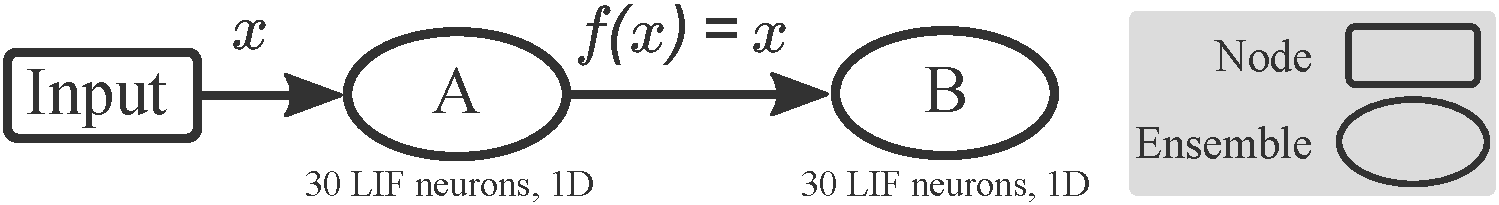
\includegraphics[width=.9\textwidth]{comm_channel}
  \begin{minipage}{0.58\textwidth}
    \begin{lstlisting}
      import nengo
      from nengo.helpers import white_noise
      model = nengo.Model("Communication Channel")
      model.make_node("Input", white_noise(1, 5))
      model.make_ensemble("A", nengo.LIF(30), 1)
      model.make_ensemble("B", nengo.LIF(30), 1)
      model.connect("Input", "A")
      model.connect("A", "B")
      model.probe("Input")
      model.probe("A", filter=0.01)
      model.probe("A.spikes")
      model.probe("B", filter=0.01)
      model.probe("B.spikes")
      sim = model.simulator()
      sim.run(1)
      A_data = sim.data("A")
      A_spikes = sim.data("A.spikes")
      ...
    \end{lstlisting}
  \end{minipage}
  \begin{minipage}{0.37\textwidth}
    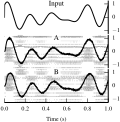
\includegraphics[width=\textwidth]{comm_channel_res}
  \end{minipage}
\end{center}
 \textbf{\refstepcounter{figure}\label{fig:cchannel} Figure \arabic{figure}.}{
   Communcation channel model. (Top) Diagram of the model.
   (Bottom left) Python code to create and run the model.
   (Bottom right) Results of the model simulation. Lines depict
   the node's output (Input panel) and the decoded value being represented
   by ensembles (A and B panels). Light gray lines in A and B panels denote
   spikes emitted by neurons in the ensembles. Each row depicts spikes
   for one neuron.}
\end{figure}

\begin{figure}
\begin{center}
  \begin{minipage}{.495\textwidth}
    \begin{lstlisting}[basicstyle={\footnotesize\ttfamily}]
      # We use Nengo to generate
      #     bias: Bias currents
      #     decoders: Decoding weights
      #     encoders: Encoding weights
      # for populations A and B.
      import pynn.nest as pyNN

      lif_params = {'tau_refrac': 2.0, 'tau_syn_E':100,
                     'tau_syn_I':100}
      dt = 0.5
      pyNN.setup(timestep=dt, min_delay=dt)
      A = pyNN.Population(30, pyNN.IF_cond_exp, lif_params)
      B = pyNN.Population(30, pyNN.IF_cond_exp, lif_params)
      input_signal = 0.5
      inputA = [pyNN.DCSource(amplitude=val) for val
                 in A_bias + input_signal * A_encoders]
      for i, pulse in enumerate(inputA):
          pulse.inject_into(A[i:i+1])
      inputB = [pyNN.DCSource(amplitude=val) for val
                 in B_bias]
      for i, pulse in enumerate(inputB):
          pulse.inject_into(B[i:i+1])
    \end{lstlisting}
  \end{minipage}
  \begin{minipage}{.495\textwidth}
    \begin{lstlisting}[basicstyle={\footnotesize\ttfamily}]
      weights = []
      for i in xrange(30):
          for j in xrange(30):
              weights.append((i, j,
                  np.dot(A_decoder[i], B_encoder[j]), 1.0))
      connection = pyNN.Projection(
          A, B, pyNN.FromListConnector(weights))
      A.record('spikes')
      B.record('spikes')
      pyNN.run(1000)

      # Decoded value of B
      B_output = numpy.zeros(1000)
      for i in xrange(1000):
          spikes = B[i:i+1].getSpikes()[:,1]
          spikes = (spikes / dt).astype('int')
          B_output[spikes] += B_decoder[i]
      # Filter with tau = 200 ms
      decay = np.exp(-dt / 200)
      B_output[0, :] *= (1 - decay)
      for i in xrange(1, 1000):
          B_output[i,:] = decay * B_output[i-1,:]
                           + (1-decay) * B_output[i,:]
    \end{lstlisting}
  \end{minipage}
\end{center}
 \textbf{\refstepcounter{figure}\label{fig:pynn} Figure \arabic{figure}.}{
   An implementation of the communication channel in PyNN.}
\end{figure}

\subsection{Lorenz attractor network} \label{sec:lorenz}

Many models in theoretical neuroscience
are based on attractor networks.
The NEF has been used in the past
to implement many different types of
attractor networks \cite{TODO}.
In this example,
we implement the Lorenz chaotic attractor
with a single ensemble
composed of 2000 leaky integrate-and-fire neurons.

\begin{figure}
\begin{center}
  \begin{minipage}{0.43\textwidth}
    \begin{lstlisting}[basicstyle={\footnotesize\ttfamily}]
      import nengo
      tau = 0.1; sigma = 10; beta = 8.0/3; rho = 28
      model = nengo.Model('Lorenz attractor')
      model.make_ensemble('State', nengo.LIF(2000),
                            dimensions=3, radius=60)

      def feedback(x):
          dx0 = -sigma * x[0] + sigma * x[1]
          dx1 = -x[0] * x[2] - x[1]
          dx2 = x[0] * x[1] - beta * (x[2] + rho) - rho

          return [dx0 * tau + x[0],
                  dx1 * tau + x[1],
                  dx2 * tau + x[2]]

      model.connect('State', 'State',
                      function=feedback, filter=tau)
      model.probe('State', filter=tau)
      model.probe('State.spikes')
      sim = model.simulator()
      sim.run(6)
    \end{lstlisting}
  \end{minipage}
  \begin{minipage}{0.55\textwidth}
    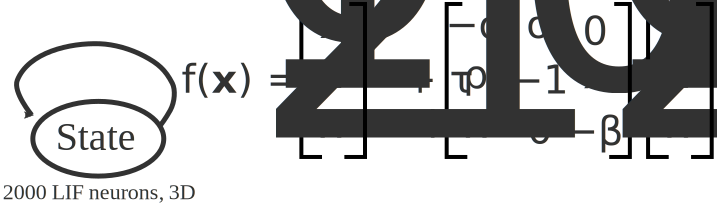
\includegraphics[width=0.95\textwidth]{lorenz}
    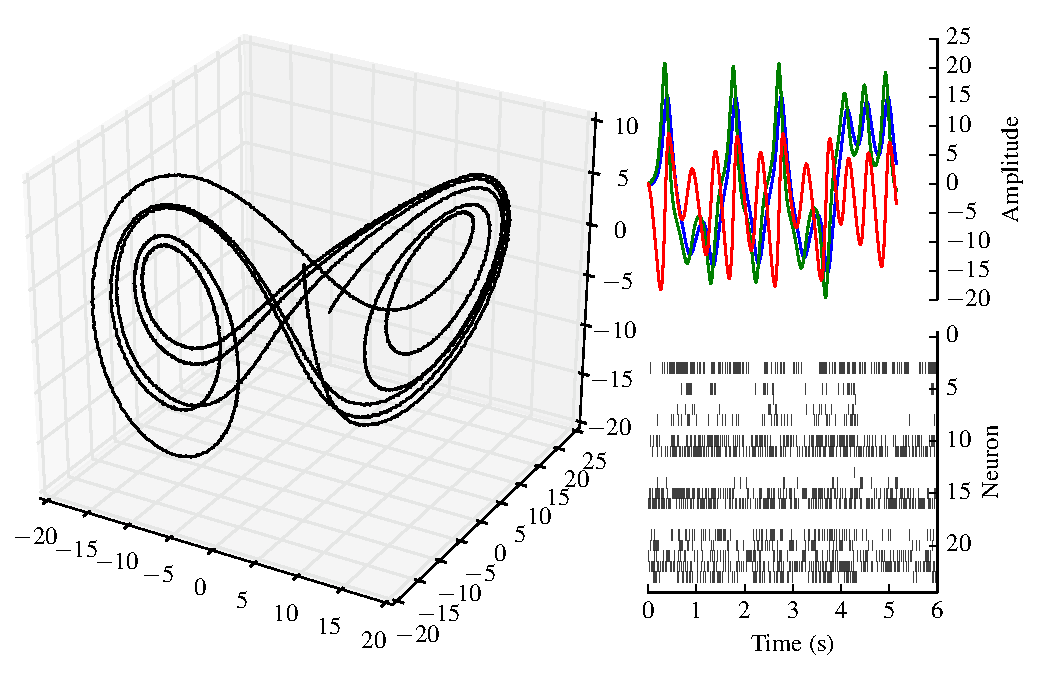
\includegraphics[width=\textwidth]{lorenz_res}
  \end{minipage}
\end{center}
 \textbf{\refstepcounter{figure}\label{fig:lorenz} Figure \arabic{figure}.}{
   Lorenz attractor model. (Left) Python code to create and run the model.
   (Top right) Diagram of the model.
   (Bottom right) Results of the model simulation. Lines depict
   the node's output (Input panel) and the decoded value being represented
   by ensembles (A and B panels). Light gray lines in A and B panels denote
   spikes emitted by neurons in the ensembles. Each row depicts spikes
   for one neuron.}
\end{figure}

In order to compare this Nengo model
with other pieces of neural modelling software,
we have implemented the Lorenz attractor
in PyNN \cite{TODO} in order to simulate it
with the simulators that PyNN supports.

\subsection{Circular convolution} \label{sec:cconv}

One of the most common operations done
in Nengo models is circular convolution.
Circular convolution is how
the semantic pointer architecture
(SPA; \cite{TODO})
binds two semantic pointers together.
Binding is central to many
of the high level cognitive tasks
that make Spaun unique.
Circular convolution
is also best implemented in a two-layer network,
rather than in a single connection.
This two-layer network construction is simplified
by the existence of the \texttt{CircularConvolution} network.

\begin{figure}
\begin{center}
  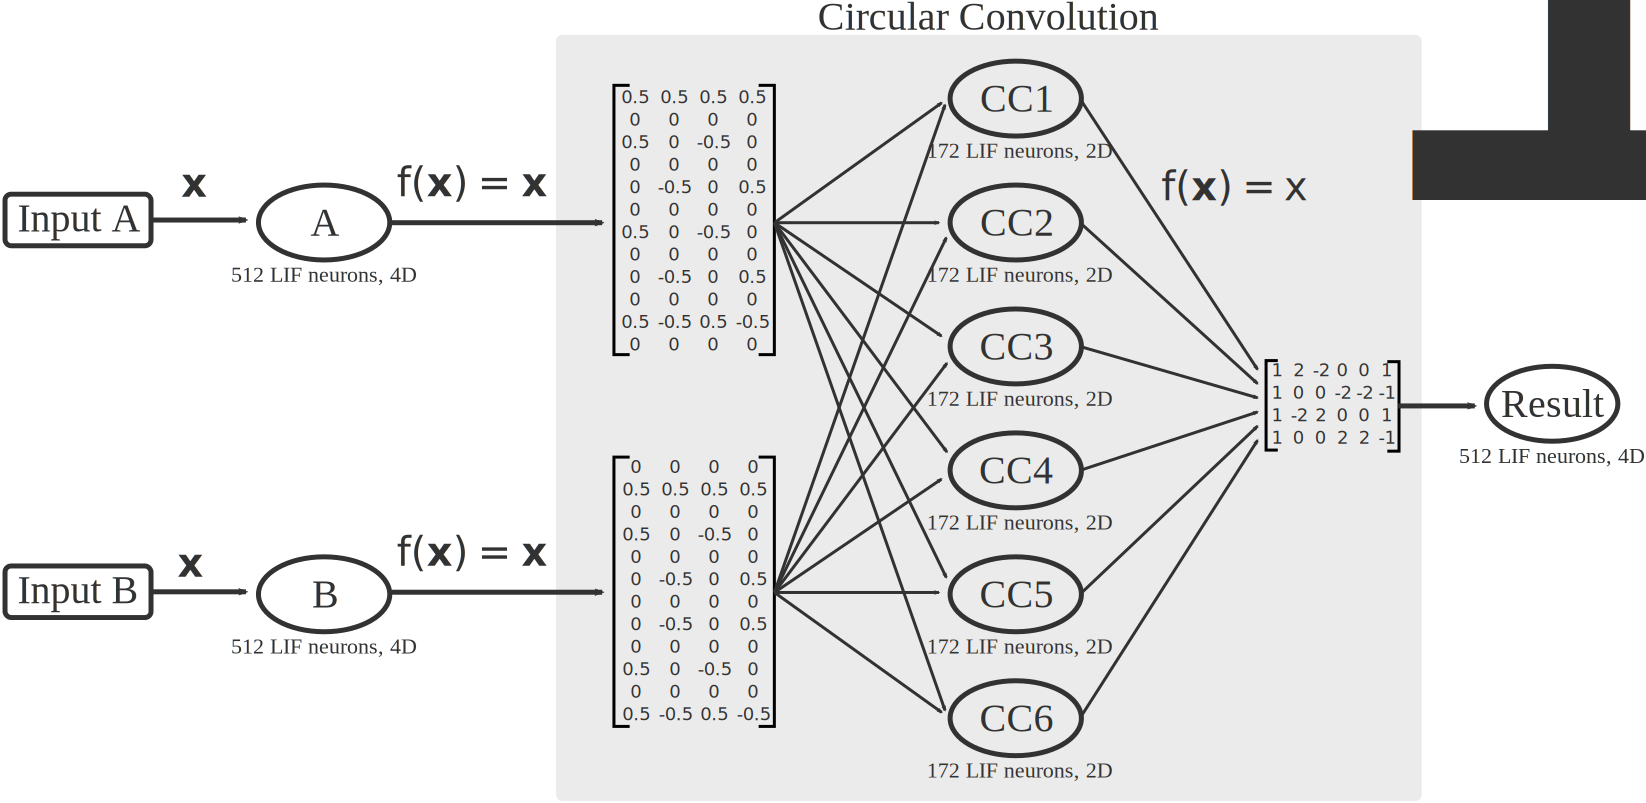
\includegraphics[width=0.8\textwidth]{cconv}
  \begin{minipage}{0.53\textwidth}
    \begin{lstlisting}[basicstyle={\footnotesize\ttfamily}]
      import nengo
      from nengo.networks import CircularConvolution
      model = nengo.Model("Circular convolution")
      model.make_node("Input A", [-0.21, 0.5, 0.12, 0.06])
      model.make_ensemble("A", nengo.LIF(512), 4)
      model.connect("Input A", "A")
      model.make_node("Input B", [-0.18, 0.28, 0.18, -0.52])
      model.make_ensemble("B", nengo.LIF(512), 4)
      model.connect("Input B", "B")
      cconv = model.add(CircularConvolution("Circular Convolution",
          neurons=nengo.LIF(1032), dimensions=4))
      model.connect("A", cconv.A)
      model.connect("B", cconv.B)
      model.make_ensemble("Result", nengo.LIF(512), 4)
      model.connect(cconv, "Result")
      model.probe("A", filter=0.02)
      model.probe("B", filter=0.02)
      model.probe("Result", filter=0.02)
      sim = model.simulator()
      sim.run(0.5)
    \end{lstlisting}
  \end{minipage}
  \begin{minipage}{0.43\textwidth}
    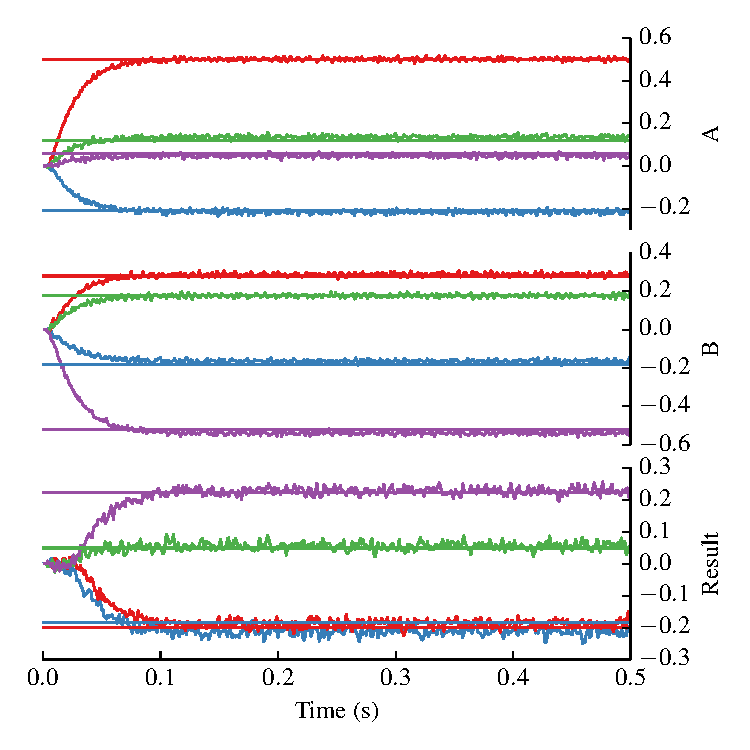
\includegraphics[width=\textwidth]{cconv_res}
  \end{minipage}
\end{center}
 \textbf{\refstepcounter{figure}\label{fig:lorenz} Figure \arabic{figure}.}{
   Circular convolution model. (Top) Diagram of the model.
   Note that much of the complexity is contained within the
   circular convolution network; the transform matrices shown
   are automatically generated by the network depending on
   input dimensionality.
   (Bottom left) Python code to create and run the model.

   (Bottom right) Results of the model simulation. Lines depict
   the node's output (Input panel) and the decoded value being represented
   by ensembles (A and B panels). Light gray lines in A and B panels denote
   spikes emitted by neurons in the ensembles. Each row depicts spikes
   for one neuron.}
\end{figure}

TODO: can we do circconv in PyNN?

\section{Benchmarks}


\begin{figure}
\begin{center}
  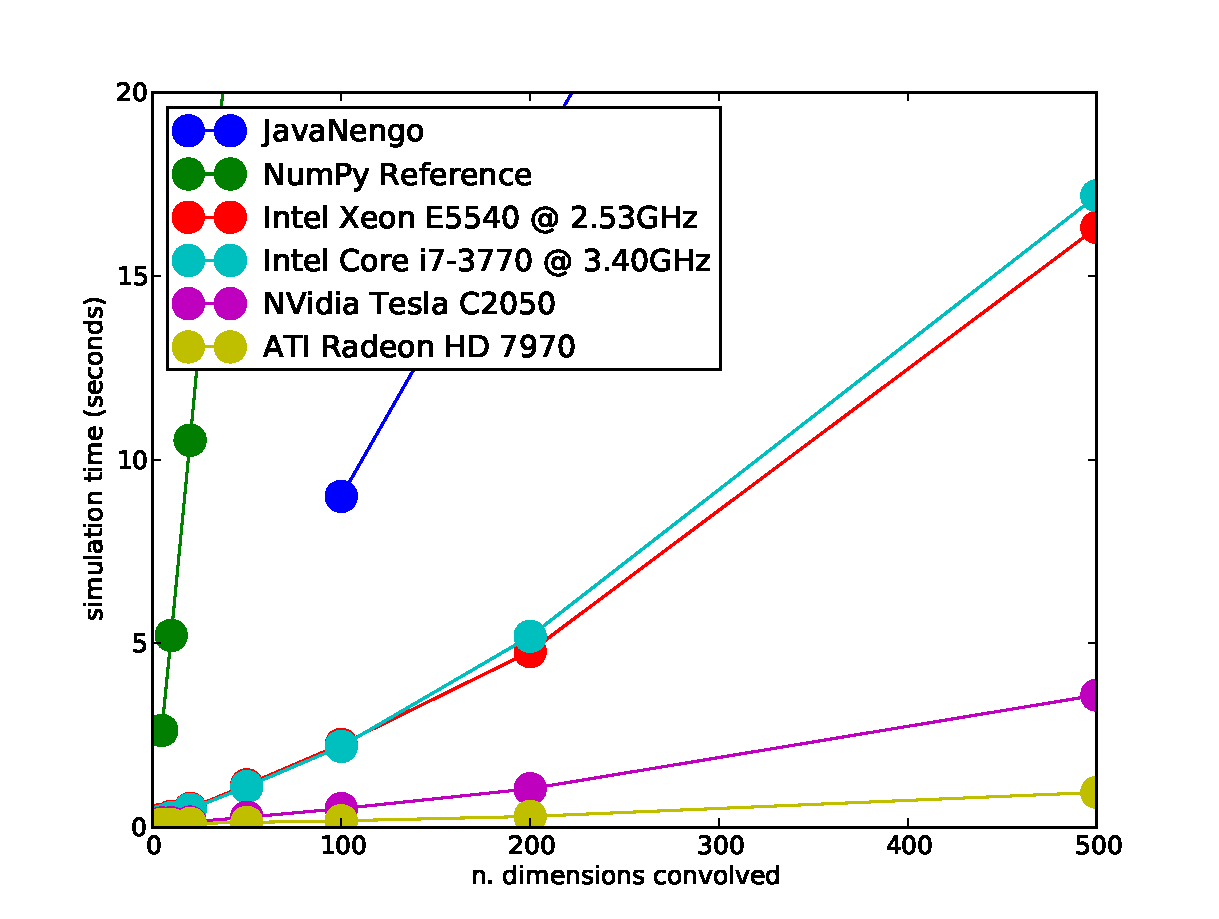
\includegraphics[width=0.5\textwidth]{ocl_vs_ref}
\end{center}
 \textbf{
     \refstepcounter{figure}\label{fig:ocl_vs_ref}
     Figure \arabic{figure}.}{
     Five-hundred-dimensional circular convolution networks were some of the most
     computationally demanding elements of the Spaun cognitive architecture.
     Simulations of circular convolution networks of various sizes illustrate the speed of our re-engineered simulators.
     A straightforward reference implementation in Python is sufficient for small networks,
     while for larger ones the new OpenCL-powered simulator runs up to 200$\times$ faster,
     In particular the Radeon 7970 GPU can simulate 500-dimensional convolution networks faster than real time (0.95 seconds for a 1-second simulation).
     Also, although both are multithreaded, our new implementation delivers better CPU performance than the previous JavaNengo implementation.
     }
\end{figure}

\section{Discussion}

Even at its \texttt{0.1} release,
we have met our goals
for this reimplementation of Nengo.
\begin{enumerate}
  \item We have provided a scripting interface
    similar to the Jython interface.
    In many cases, the new scripting interface
    is simpler and more expressive than
    the previous Jython interface.
  \item We have leveraged existing scientific computing tools
    rather than writing our own.
    In the the scripting interface and the reference simulator,
    we use NumPy to simplify array computations.
    In the reference simulator, we use
    NetworkX to perform the topological sort
    of the operator dependency graph.
    In examples, we use Matplotlib
    to plot the results of simulations.
  \item We have provided the ability to run models with
    different software and hardware simulators.
    We have shown that this is possible by
    implementing two software simulators.
\end{enumerate}

While this reimplementation of Nengo
does not completely replace
the existing suite of Java-based Nengo tools,
it is able to cover the vast majority of use cases
with an order of magnitude less
code than the Java-based tools
($\sim$30,000 lines of Java + 10,000 lines of Jython
vs. $\sim$8,000 lines of Python).
We are optimistic that the remaining use cases
can be implemented in this new framework.

TODO: something about documentation, unit tests,
coverage, travis-ci, etc

\subsection{Comparison to similar projects}

There are many other neural simulators
dedicated to building large-scale neural models;
however, Nengo is unique in being built
on a theoretical framework (the NEF, \cite{TODO})
that has already been used to make
large-scale functional brain models.

The most closely related project is PyNN
\cite{TODO},
which provides a high-level scripting
interface similar to the
model creation part of Nengo.
Rather than implementing its
own simulator, PyNN uses existing
simulators, such as Brian \cite{TODO},
NEST \cite{TODO}, and NEURON \cite{TODO}.

The APIs of Nengo and PyNN are similar,
but differ significantly
in how groups of neurons are connected together.
In Nengo, connections commonly describe
the mathematical operation that is performed
through the connection between
two ensembles;
e.g., \texttt{DecodedConnection(A, B,
function=product)} connects ensemble A
to ensemble B, projecting the product of
some dimensions encoded by A to B.
In PyNN, connections commonly describe
features of the connection weight matrix
between two populations;
e.g., \texttt{FixedProbabilityConnector(0.5)}
connects two ensembles together,
with a probability of 0.5
that there will be a connection
between a pair of neurons in the two populations.

As shown in Figure~\ref{TODO},
Nengo is able to simulate many networks
faster than all of PyNN's simulators
(TODO: right?).
This is, in part, because Nengo stores two vectors
whose product is the entire
connection weight matrix between
two ensembles, rather than storing
the entire matrix.

However, PyNN also contains functionality
not currently implemented in Nengo.
PyNN can assign spatial information
to neurons in a population,
which can be used to influence
how those neurons connect to other populations.
PyNN simulates many different learning rules
and neuron types,
and is therefore better suited to
simulate small networks of detailed neuron models
(as would be necessary for modelling
an invertebrate nervous system).

\subsection{Future work}

Nengo is a young project that
has started with a deliberately minimal base
in order to make contributing easier than in
previous implementations.
Additionally, many neural modellers
are already using Python,
as evidenced by the existence of
PyNN, Brian, and Python bindings to other simulators.
Nengo will be able to benefit
from improvements to scientific Python tools.
It is also extendable by modellers with
varying technical skills;
creating a new network is simple,
while creating a new simulator is complex.

By enabling outside contributions,
and providing a user friendly API
and many example models,
we hope to foster a rich community of modellers
contributing networks, nonlinearities,
and simulators to Nengo
and to theoretical neuroscience
as a whole.

\section*{Disclosure/Conflict-of-Interest Statement}

The authors declare that the research was conducted in the absence of
any commercial or financial relationships that could be construed as a
potential conflict of interest.

\section*{Acknowledgement}

We would like to thank
everyone who has contributed
to this reimplementation of Nengo
by providing examples,
unit tests, and bugfixes:
Peter Blouw, Brent Komer, and Bryan Tripp.

\paragraph{Funding\textcolon}
NSERC CRC, CFI, and OIT.

\bibliographystyle{frontiersinSCNS&ENG}
\bibliography{nengo}

\end{document}
